\chapter{Background}\label{chapter2}


\section{Cosmic fields: Characterizing non-linear growth of Cosmic structure}
% Taken from Comprehensive essay
% /home/nes/MEGA/Google_drive/KU courses/Fall2016/CompreEssay/Compre1/draft_compre_clean.tex


The most fundamental attributes of particles in the N-body simulations are their position and velocity co-ordinates, and their masses. Due to the lack of numerical tools for direct analysis these raw data, fields such as mass density $\rho(\mathbf{x}, t)$, velocity $\mathbf{v}(\mathbf{x}, t)$ or gravitational potential $\phi(\mathbf{x}, t)$ fields are often computed numerically. Mass density fields were calculated using Cloud-in-Cell (CIC) algorithm (cf. \citealt{Hockney1988}), which is numerically equivalent to counting the number of particles on each cell of a regular grid. Alternatively, the density field also generated on irregular grids by applying Delaunay (For example, \citealt{Icke1991} and the Delaunay Tessellation Field Estimator (DTFE) by \citealt{Schaap2000} and \citealt{Weygaert2009a}) or Voronoi tessellations (See \citealt{Schaap2000} and references therein) to the particle coordinates. Another parameter `linking length', using distances between nearest neighbouring particles, was used for percolation analyses and identifying super-clusters of galaxies ( \citealt{Zeldovich1982}, \citealt{Shandarin1983} and \citealt{Shandarin1983b}) for identifying halos \citealt{Davis1985} in the cosmological simulations. Left panel in \autoref{fig:cosmicfields} shows some of the popular fields/parameters that use particle mass and positions. It has to be noted that the density fields or linking-lengths are not dynamical descriptions that invoke the initial field of density fluctuations or the velocity of the particles. 


\begin{sidewaysfigure}
\begin{minipage}[t]{0.99\linewidth}
 \centering\includegraphics[height=10.5cm]{Chapter1/Plots/fig0.pdf} 
\end{minipage}\hfill
\captionsetup{font={small,stretch=1}}
\caption{Classification of some of the fields/parameters used in cosmological analyses. Some fields utilise position co-ordinates only whereas others use the full phase-space information. In addition, the fields may be defined on a regular grid, or may be defined on an unstructured grid (For instance, flip-flop is a number-valued field defined on each dark matter particle). Fields like mass density and multi-streams can be defined on either grids, depending on the numerical technique. List is obviously not exhaustive- velocity and potential fields are not included, and discussions of correlation functions are excluded as well.}
\label{fig:cosmicfields}
\end{sidewaysfigure}


An obvious advantage of methods based on particle coordinates, both on structured and unstructured grids, is their applicability to redshift catalogues. The redshift catalogues like SDSS and 2dF provide only two angular coordinates and distances in redshift space. But cosmological N-body dark matter simulations provide the full dynamical information in six-dimensional phase space. This additional information is very valuable providing a greater opportunity for understanding the physics of the web and developing a better theory of the web.


The velocity fields in the simulations of collision-less cold dark matter particles can become multi-valued under the action of gravity. This phenomenon was first discussed by \cite{Zeldovich1970}, where he predicted the formation of non-linear structures (also see \citealt{Shandarin1989} for discussion on formation of multi-stream). The primordial oblate structures were later known as `Zel'dovich pancakes'. These pancakes grow from initial perturbations in a continuous mass distribution, where the velocities are single-valued (also referred to as single-stream) everywhere in the configuration space. Multiple values in the velocity field $\mathbf{v} (\mathbf{x},t)$ or `multi-streams' can also be seen in the dynamically equivalent Lagrangian sub-manifold - $(\mathbf{q}, \mathbf{x})$, where $\mathbf{x}$ and $\mathbf{q}$ are co-moving Eulerian and Lagrangian co-ordinates respectively. \cite{Shandarin2011} and \cite{Abel2012} studied this $ \mathbf{q} \mapsto \mathbf{x}$ mapping in N-body simulations to quantify the number of streams using phase-space tessellations. \cite{Shandarin2011} define a multi-stream field $n_{str}(\mathbf{x})$ as a field taking discrete values that are equal to the number of streams at every evaluation point in configuration space. Ordered sign-reversal of each elementary volume element in the Lagrangian sub-manifold was measured by \cite{Shandarin2014a}. Their {\it flip-flop} field $n_{ff}(\mathbf{q})$ in Lagrangian space demonstrates a very rich sub-structure of the cosmic web, especially in a halo environment. 

Fields computed from a complete dynamical information (either $(\mathbf{q}, \mathbf{x})$ or $(\mathbf{p}, \mathbf{q})$) could provide valuable contributions to our understanding of the cosmic structure. \cite{Falck2012} have recently delineated archetypal web structures by counting the number of foldings in the sub-manifold for each dark matter particle along different directions. Another study by \cite{Ramachandra2016a} explored some of the global topological and local geometrical properties of the web in the context of multi-streaming. The applications of these analyses is certainly not limited to diagnostic tools; the multi-streaming phenomenon can be used in improving N-body simulations \citep{Hahn2013}, and studying galaxy evolution and star formation as well \citep{Aragon-Calvo2016}. 



\section{Zel'dovich Approximation}
% Taken from the Caustics paper

\label{sec:ZA}

ZA is an elegant analytical approximation to describe the non-linear gravitational evolution of collisionless particles in continuous media. Technically it is the first oder Lagrangian perturbation theory, however Zeldovich suggested to extrapolate it to the beginning of the non-perturbative nonlinear stage and predicted the formation of caustics which are the boundaries of
the first very thin multistream regions dubbed by him  'pancakes'.
ZA describes a dynamical mapping from the initial Lagrangian coordinates $\mathbf{q}$ to Eulerian positions at time $t$. In comoving coordinates, $\mathbf{x} = \mathbf{r}/a(t)$ (where $\mathbf{r}$ is the physical coordinate  and $a(t)$ is the scale factor; assuming normalization $a(z=0)=1, \mathbf{r}$ are 
the physical coordinates of particles at present ), ZA takes the form:

\begin{equation} \label{eq:ZA1}
 \mathbf{x}(\mathbf{q}, D(t) ) = \mathbf{q} + D(t) s(\mathbf{q}) 
\end{equation}

where $D(t)$ is the linear density growth factor, and the the initial density perturbation field $\psi(\mathbf{q})$ determines the potential vector field $\mathbf{s(q)} = - \nabla_q \psi(\mathbf{q})$. 
% The initial cosmic density field is a realization of a Gaussian random process, specified completely by the associated power spectrum, $P(k)$. 
Mass conservation formalism implies $\rho(\mathbf{x}, t) d\mathbf{x} = \rho_0 d\mathbf{q} $, so the density field at $t>0$ in terms of Lagrangian coordinates is given as 

\begin{equation}
 \rho(\mathbf{q}, t) = \rho_0 J \left[ \frac{\partial\mathbf{x}}{\partial\mathbf{q}} \right]^{-1}
\end{equation}

where the Jacobian $J \left[ \frac{\partial\mathbf{x}}{\partial\mathbf{q}} \right]$ is calculated using Equation \ref{eq:ZA1}. Moreover, diagonalization of the resulting real, symmetric deformation tensor $d_{ij} = - \nabla_q \mathbf{s(q)} =  \partial^2 \psi(\mathbf{q})/ \partial q_i \partial q_j$ in terms of its eigenvalues $\lambda_1(\mathbf{q})$, $\lambda_2(\mathbf{q})$, $\lambda_3(\mathbf{q})$ gives the contraction or expansion along the three principal axes. This reduces the mass density to a convenient form:

\begin{equation}
 \rho(\mathbf{q}, t) = \frac{\rho_0}{ \left[1 - D(t) \lambda_1(\mathbf{q}) \right]\left[1 - D(t) \lambda_2(\mathbf{q}) \right]\left[1 - D(t) \lambda_3(\mathbf{q}) \right] }
\end{equation}

Since the deformation tensor $d_{ij}$ and its eigenvalues depend only on the initial density field, the ordered eigenvalues defined in Lagrangian space $\lambda_1(\mathbf{q}) \geq \lambda_2(\mathbf{q}) \geq \lambda_3(\mathbf{q})$ determine collapse condition for masses in Eulerian space (see \cite{Doroshkevich1970} and \cite{Lee1998} {for the PDFs  of the eigen values as well as several other parameters} in the case of Gaussian random fields). In the context of this paper, formation of caustics is of much interest: with increasing $D(t)$, the mass density rises until reaching singularity at $D(t) = 1/\lambda_3(\mathbf{q})$. In Lagrangian space, the caustics stem from these points and their counterparts  in Eulerian space were proposed by Zel'dovich as the 'birthplaces' of the first collapsed structure by gravitational clustering. Now the regions bounded by the caustic surfaces are referred to as {\it Zel'dovich pancakes}. The collapse along other principal axes correspond to formation of filaments and knots \citep{Arnold1982}, Shandarin and Klypin (1984). However simultaneous collapses along all three eigen axes never happen in the case of generic flows.

\begin{figure} 
\centering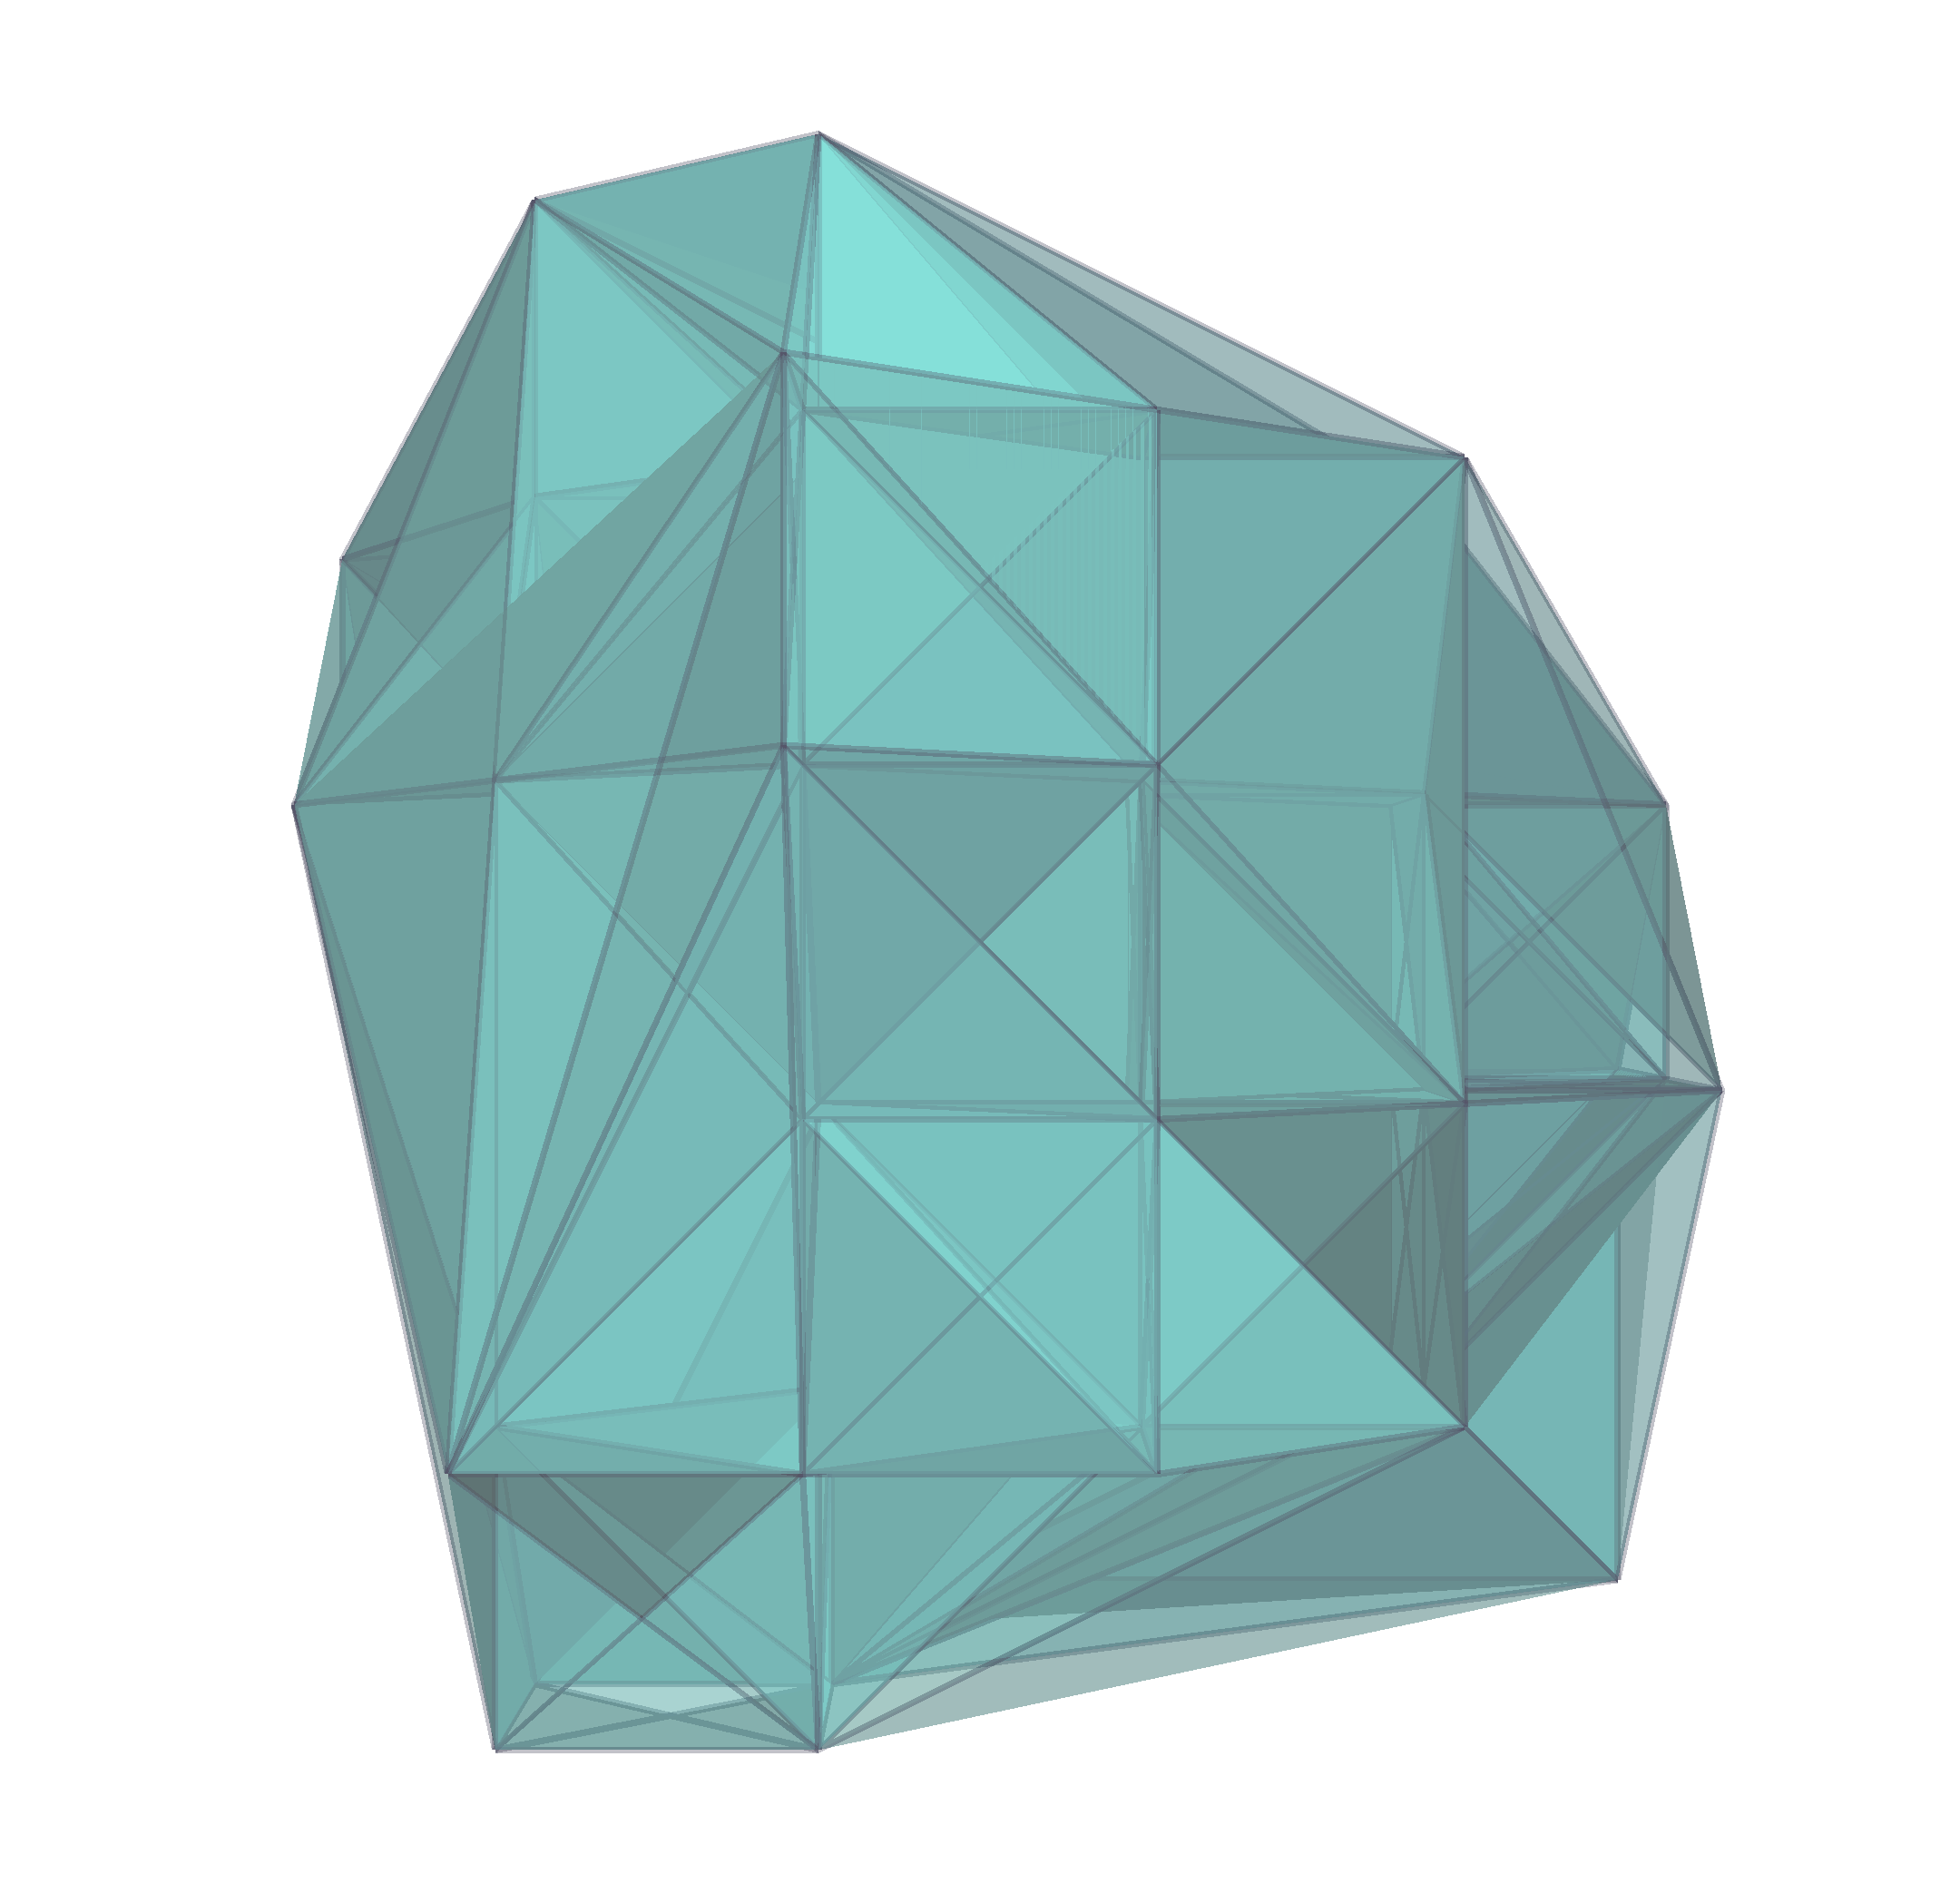
\includegraphics[width=8cm]{Chapter2/Plots/qDel.png}
\centering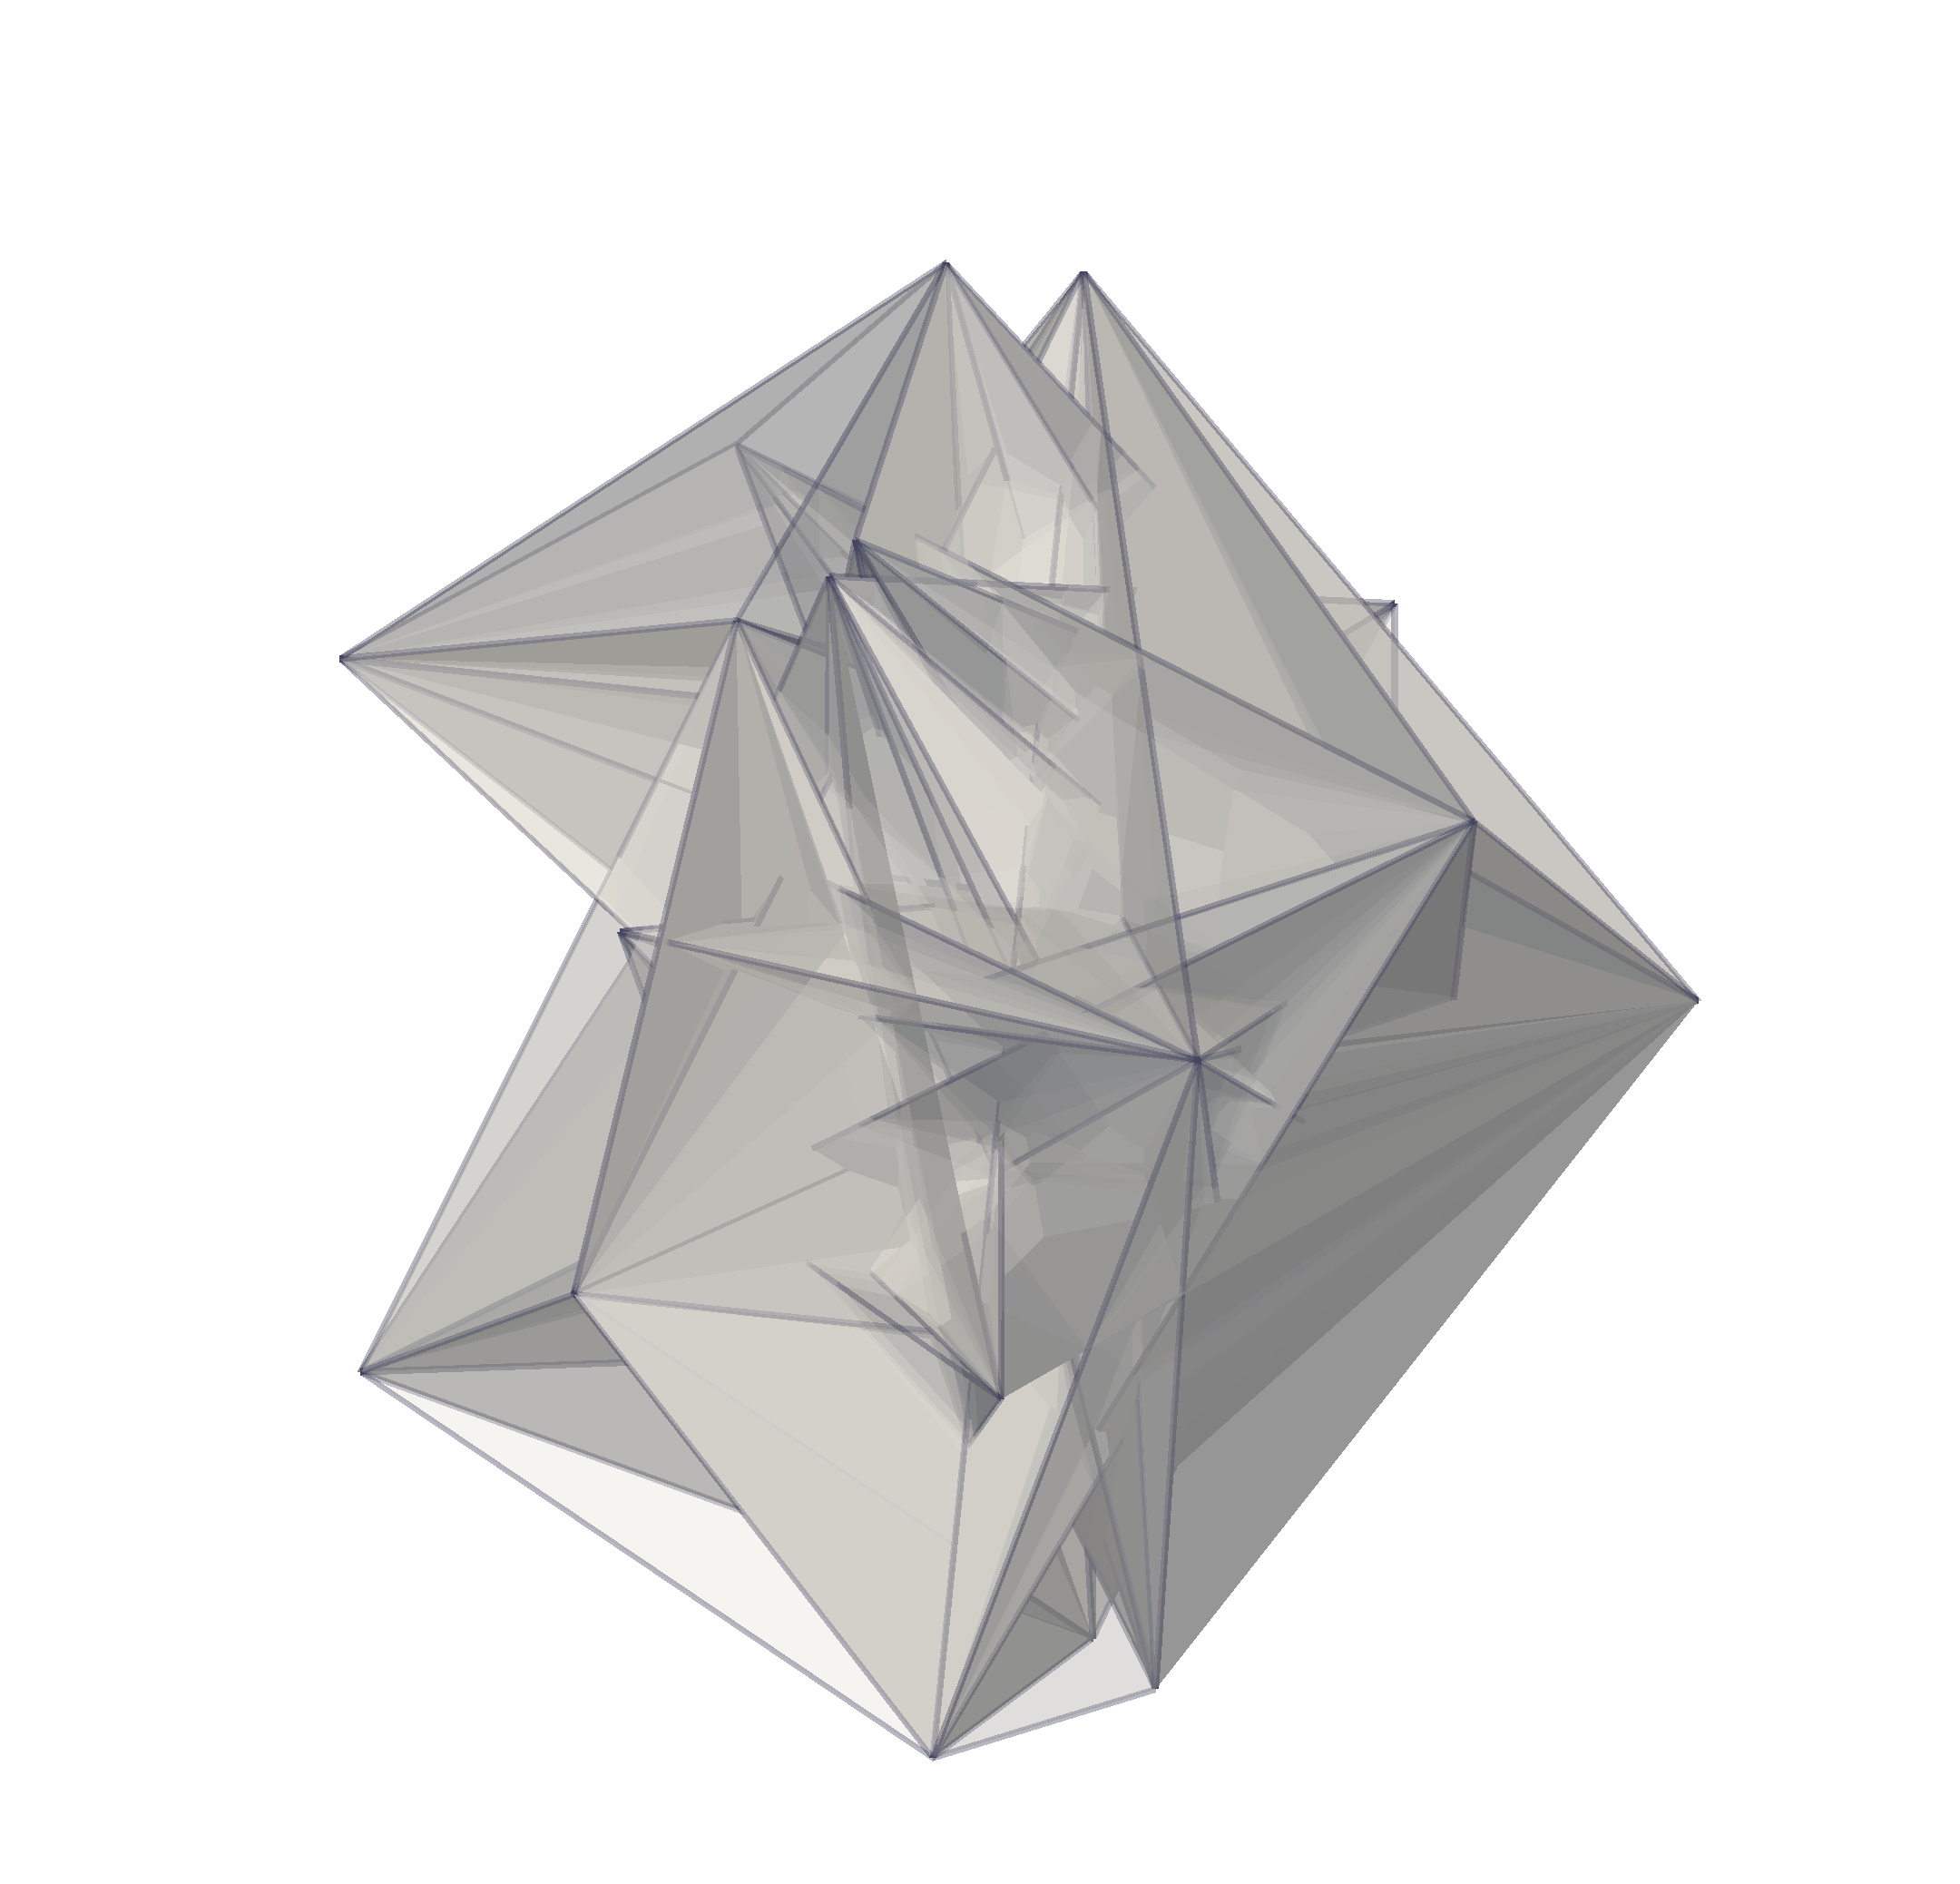
\includegraphics[width=6cm]{Chapter2/Plots/x.png}
\caption{ This plot shows the idea of Lagrangian tessellations. Left: The distribution of Dark matter particles in Lagrangian space is on the regular grid. The tetrahedra surfaces in this case are mostly regular (except at the edges). Right panel shows the Eulerian positions of the same particles at $z=0$. The particles clearly have undergone multiple flip-flops, and the intersections of Lagrangian tetrahedra signifies locations of caustic surfaces. Specific tessellation schemes can be utilized separately to identify these surfaces. }
\label{fig:Tess}
\end{figure}


Furthermore, the analytical understanding of these structures are thoroughly complicated: In a 2-dimensional ZA, for example, there are only two types of fundamental singularities that exist at generic instants of time($A_2$, which are lines and $A_3$, which are the cusp points of $A_2$ lines).   In addition there are two singular points ($A_4$, and $D_4$) that exist  only at particular instants of time: at $A_4$ two cusp $A_3$-points are formed and a smooth part of an $A_2$ line is  transformed in self-crossing
line. In addition there are several transient forms that exist only 
at particular times.
Each of these correspond of formation, mergers, branching and other dynamical processes involving pancakes. \cite{Arnold1982} and \cite{Hidding2014} studied of singularities in 2-dimensional collapse) in exhaustive detail, but similar analytical characterization of 3-dimensional ZA has not been satisfactorily done yet.  
 
 
Complexities in 3-dimensional caustics is partly due the intricate mapping in the hypersurface $\mathbf{x}(\mathbf{q})$ called the Lagrangian submanifold (See Figure \ref{fig:Tess}). The Lagrangian submanifold $\mathbf{x}(\mathbf{q})$  is a single valued, smooth and differentiable function in it's 6-dimensional space $(\mathbf{q}, \mathbf{x})$, however the projection onto 3-dimensional Eulerian space is entangled with creases, kinks and folds (Note that this  submanifold is very different than the phase space $(\mathbf{x},\mathbf{v})$, even though they are connected by a cannonical transformation). However, dilineating the Lagrangian submanifold reveals several properties of the dark matter dynamics not inferred from position-space analyses. Two fields related to tessellating the Lagrangian submanifold -- The Multistream field $n_{str}(\mathbf{x})$ in Eulerian space and the Flip-Flop field $n_{ff}(\mathbf{q})$ in Lagrangian space (check \cite{Shandarin2012}, \cite{Ramachandra2015}, \cite{Shandarin2016}) are closely related. 





\section{The multistream flow field in one-dimension}
% Taken from appendix A
\label{appendix:nstream}

\begin{figure}
\begin{minipage}[t]{.99\linewidth}
  \centering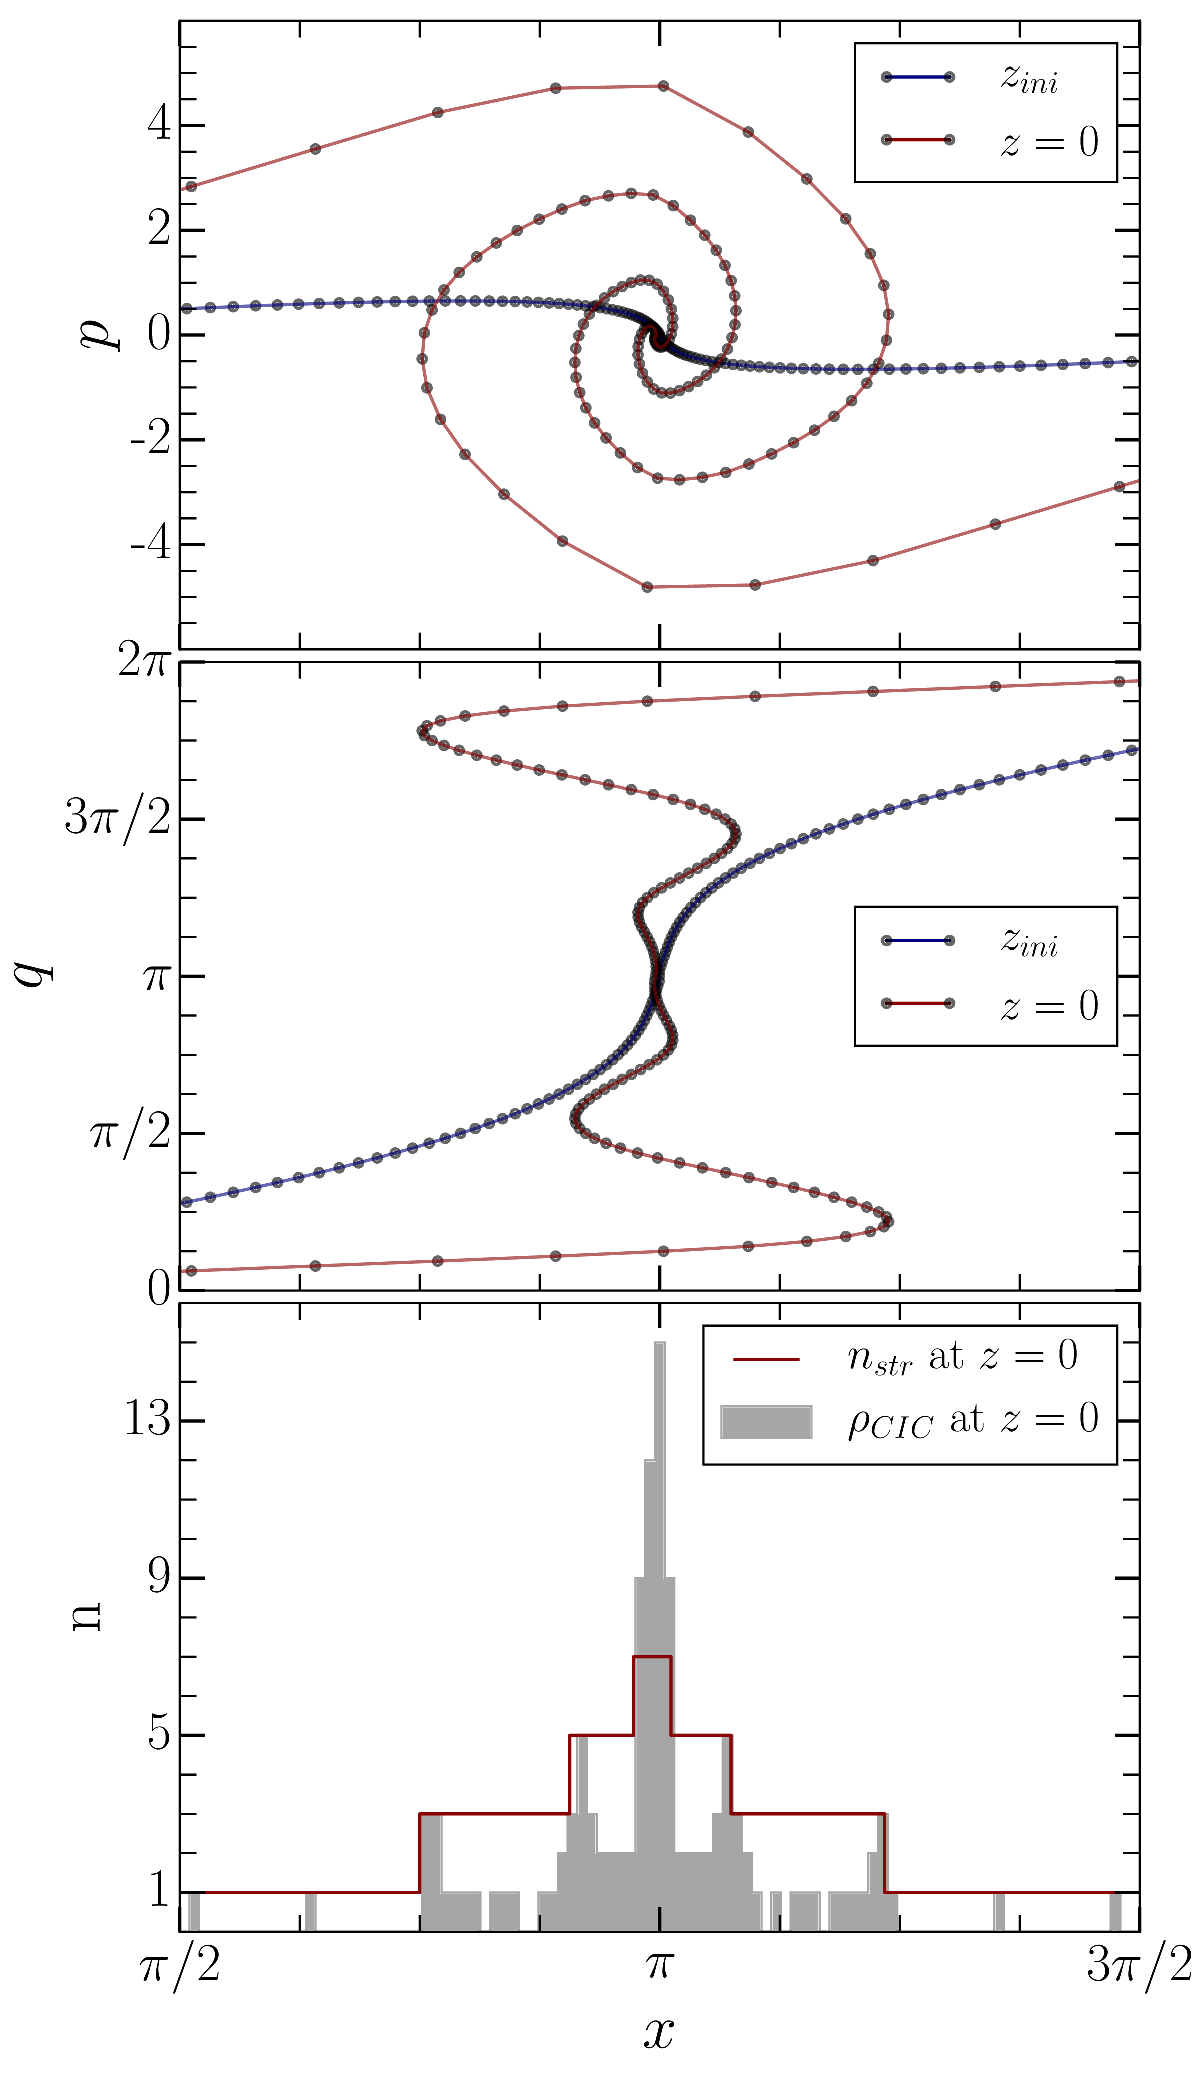
\includegraphics[width=8.cm]{Chapter4/Source_v2/fig13.pdf} 
\end{minipage}\hfill
\caption{ Multi-streaming in one-dimension gravitational collapse. Top panel: $(\bf{p}, \bf{x})$ phase-space representation redshift $z_{ini}$ and $z = 0$. Dots represent the dark matter particles. Initially the mass particles are in the linear stage of evolution. At $z = 0$, multiple values of $\bf{p}(\bf{x})$ is seen in the collapsed regions. Middle panel: Equivalent Lagrangian sub-manifold $\bf{q}(\bf{x})$. At $z_{ini}$, the dashed line represents $\bf{q} = \bf{x}$. Number of streams are parametrized from this sub-manifold. Bottom panel: The multistream field $n_{str}$ and the number-density using CIC algorithm, $n_{CIC}$ at $z = 0$. }
\label{fig:phase1d}
\end{figure}

The top panel in \autoref{fig:phase1d} shows the velocity multistreaming phenomenon in a one-dimensional collapse. The phase-space $(\bf{p}, \bf{x})$ (where $p$ is the momentum and $x$ is the co-moving Eulerian coordinate) is single-valued in the linear stage of evolution (at redshift $z_{ini}$). Non-linear stage of gravitational evolution of the collision-less dark matter particles then results in multi-valued $\bf{p} (\bf{x},z)$ at $z = 0$. The mass particles are sparsely  distributed outside the region of gravitational collapse, and are denser in the inner streams.

 
A dynamically equivalent transformation $(\bf{p}, \bf{x}) \mapsto (\bf{q}, \bf{x}) $ (where $\bf{q}$ is the Lagrangian coordinate) shows the Lagrangian sub-manifold in the middle panel of \autoref{fig:phase1d}. This two-dimensional phase-space has foldings that correspond to multiple velocity streams, although the sub-manifold itself remains continuous. A projection of the Lagrangian sub-manifold at each point in the configuration space quantifies the number-of-streams. Folding in the sub-manifold are checked for points in configuration space using tessellations. The tessellating simplices in one-dimensional model are just the line-segments whose nodes are the dark matter particles in the Lagrangian space. Dynamical property is accounted for in this phase-space tessellation since labels of the nodes remain intact throughout the evolution; the line segments may shorten, extend or change orientation. Each folding in the Lagrangian sub-manifold increases the number of streams by a factor of two. In three-dimensional simulations, the sub-manifold twists in complicated ways in a six-dimensional phase space. The number-of-streams in N-body simulations (\citealt{Shandarin2012} and \citealt{Abel2012}) is calculated using Lagrangian/phase-space tessellations. This triangulation is conceptually different from the Voronoi (See \citealt{Schaap2000} and references therein) or Delaunay \citep{Icke1991} tessellation schemes. 

The bottom panel \autoref{fig:phase1d} shows the the multistream field $n_{str}(\bf{x})$ at $z = 0$. The field only takes the values of 1, 3, 5 and 7 in this scenario. Caustics occur at the folds in Lagrangian sub-manifold, and have a measure zero (study of caustics in one- and  two-dimensional evolution is done in \cite{Hidding2014}, three-dimensional caustic surface in a cosmological simulation is shown in \cite{Ramachandra2017} ). Several properties of the multistream field are significantly different from mass density. The bottom panel also shows an illustration of CIC algorithm (cf. \citealt{Hockney1988}) in calculating density, which is numerically equivalent to counting the number of particles on each cell of a regular grid. One major difference is in the regions before gravitational collapse: $n_{str}$ is universally equal to unity, whereas number density fluctuates. It should also be noted that density by definition is a continuous field; numerical approximations like CIC discretise the field. Alternatively, multistream field is intrinsically a discrete-data field.  



%-------------------------------------------------------------------------------------------------------------------------------
\section{Phase-space representation of gravitational clustering}
\label{sec:HaloFormation}
%% Taken from Paper2017b

\begin{figure*} 
\centering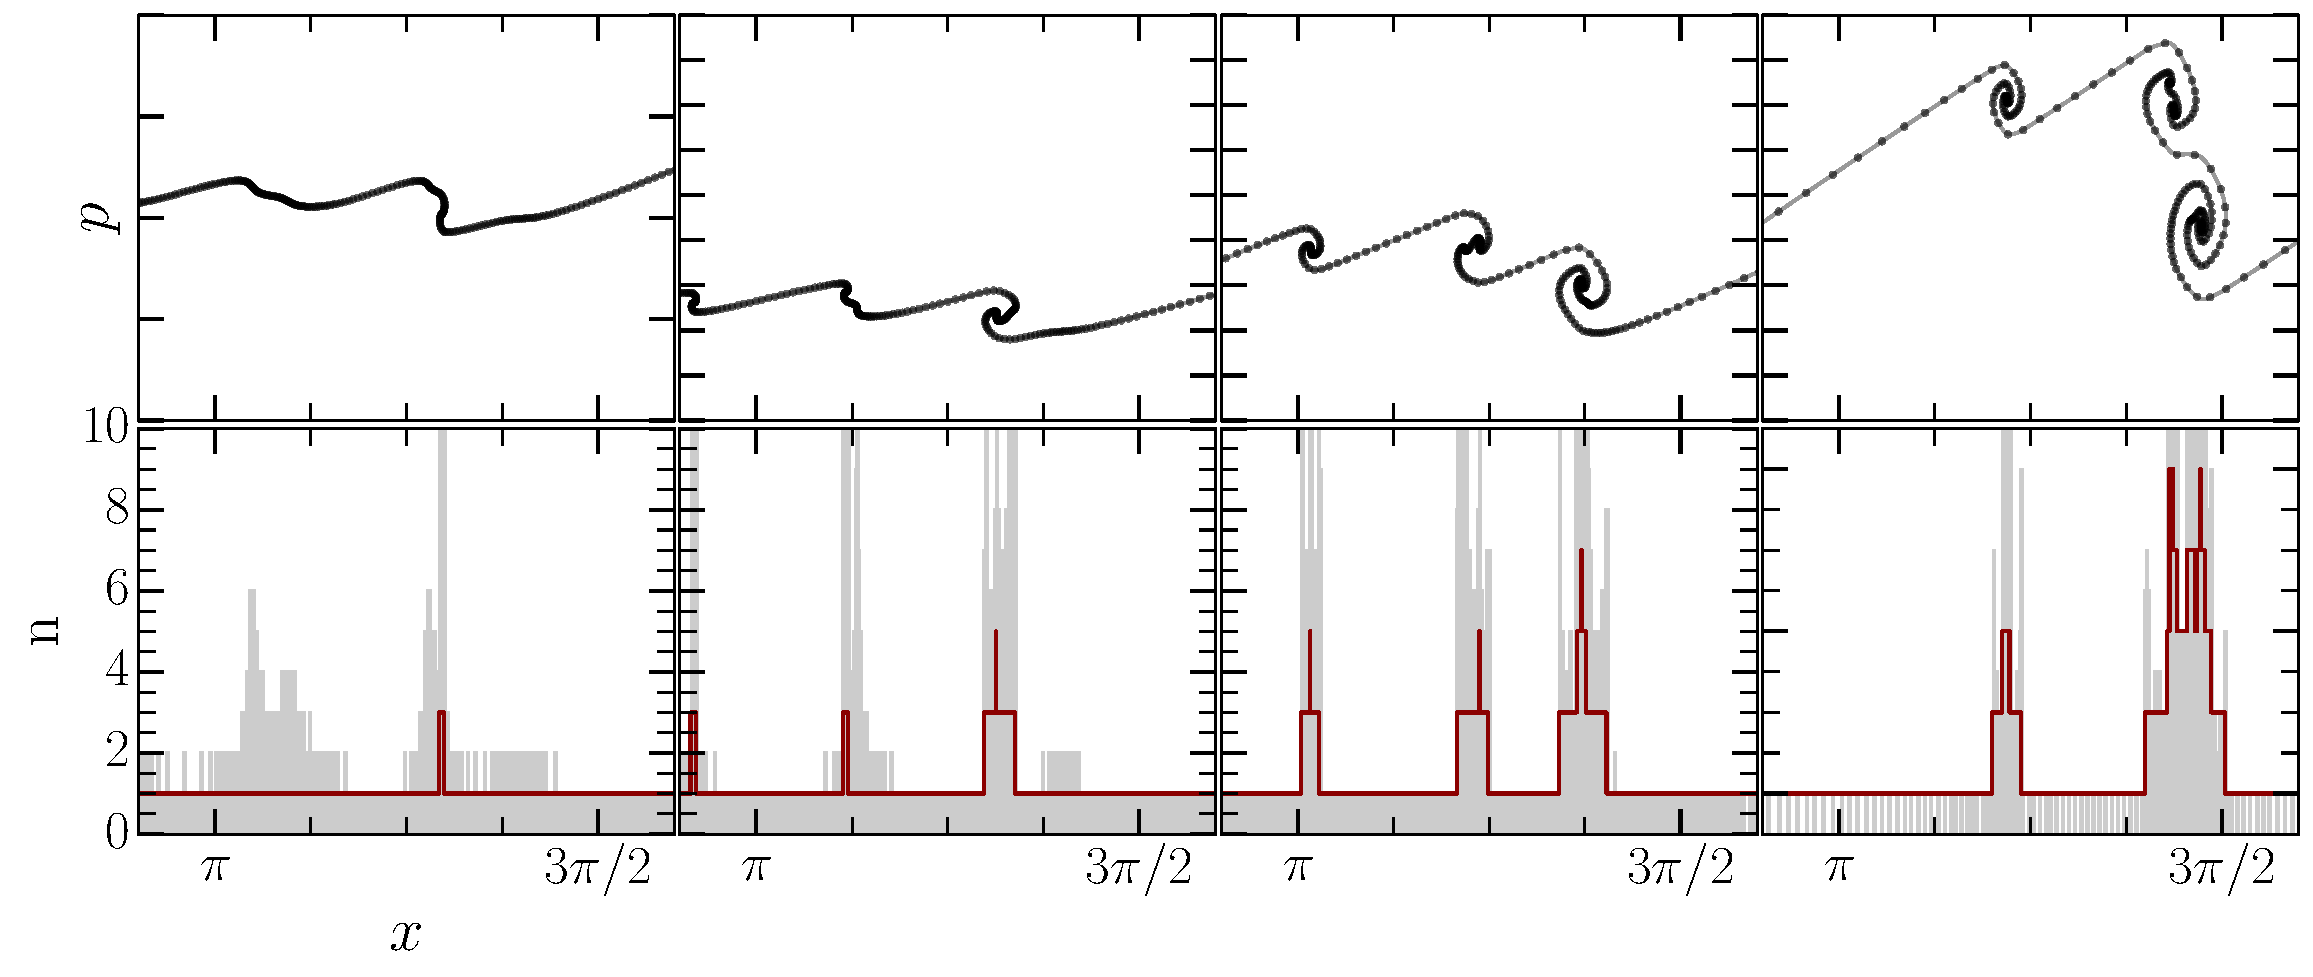
\includegraphics[height=7cm]{Chapter5/Source_v2/fig1.pdf} 
\caption{Dynamical collapse of dark matter in one-dimensional universe: Top panels show the $(\mathbf{p}, \mathbf{x})$ phase-space manifold of the dark matter sheet at redshifts $z_1$, $z_2$, $z_3$ and $z = 0$. Dots represent the dark matter particles. The momentum values are chosen at arbitrary scales. Bottom panels show the corresponding multistream field multistream field $n_{str}(\mathbf{x}, z)$ (red) and density field $\rho(\mathbf{x}, z)$ (gray). }
\label{fig:1d}
\end{figure*}

We begin with a simple illustration showing the formation of a few haloes in a one-dimensional simulation. Dark matter clustering in a (1+1)-dimensional phase-space $(\mathbf{p}, \mathbf{x})$ (where $p$ is the momentum and $x$ is the co-moving Eulerian coordinate) at four successive time steps is shown in the top panels of \autoref{fig:1d}. The lower panels show the corresponding multistream field (\citealt{Shandarin2012} and \citealt{Abel2012}) $n_{str}(\mathbf{x}, z)$ (red) and density field $\rho(\mathbf{x}, z)$ (gray). At $z_1$ (left-most panel), velocity is single-valued in Eulerian co-ordinates shown, except at a small three-stream region near $\mathbf{x} = 5\pi/4$. This is the first instance of multistreaming in the region, which was previously had $n_{str} = 1$ throughout. The interface of $n_{str} = 1$ and $n_{str} = 3$ regions is also the location of the first caustic. On the other hand, the density calculated at a high resolution shows variations, even in the mono-streaming regions. The variations are especially more pronounced around  the caustic (near $\mathbf{x} = 5\pi/4$).


The gravitational clustering is more evolved in the two center panels ($z_2$ and $z_3$) with three prominent phase-space spirals. The regions between the spirals have sparsely distributed dark matter particles, and have $n_{str} = 1$. Each spiral corresponds to a location of gravitational collapse with $n_{str} > 1$ region, and higher density. A few of these regions within three-streaming regions are elevated to $n_{str} = 5$. The corresponding density field is not only noisier, but also reaches very high values at the caustics. This is also a primary distinguishing feature between mass density fields and multistream fields: At the locations of caustic, the density (regardless of how it is calculated) is not smooth \cite{Vogelsberger2011}. Computational limitations on simulation resolutions and refinement of density calculations soften the fields, exceptionally at the zero volume measure regions of caustic surfaces.  On the other-hand, multistream values are increased by finite values at caustic surface locations - This property is preserved at higher simulation resolutions and any refinements of multistream field calculations - although $n_{str}$ may be resolved enough to have intermediate even-values. Multistream fields are also intrinsically discrete valued, which is not true with density fields. Discreteness of multistream fields is discussed in more detail in \cite{Ramachandra2017}. 

The right-most panel in \autoref{fig:1d} shows the final structure at $z=0$. Two large spirals have spatially merged. These collapse environments are naturally very complex, with an increased number of successive caustic formation and merging. 
The corresponding velocity streams also show a more complicated structure. Clearly, the multistream field has a saddle point that is not as low as $n_{str} = 1$. This poses a bigger problem in the context of most of halo detection algorithms, and we discuss this in Appendix \ref{appendix:Eigen}. 



\subsection{Collapse in higher dimensions}

Extending the above results of one-dimensional collapse into higher dimension is vital, primarily in the context of halo formation. The individual spiral collapses in the one-dimension happen at a small region (left-most panel in \autoref{fig:1d}), and the region grows by volume, whilst increasing the spiral twists within. This is in contrast with the theoretical top-hat spherical model of halo formation when the shell crossing would not happen until the final moment of the collapse of the entire halo into a point-like singularity. Thus all shell crossings happen at a single point
and at a single instant of time. The collapse of an isolated, spherically symmetric density peak is a very exceptional case, because every spherical shell feels only the force due to interior mass until it collapses into the caustic region. The collapse of the real peak proceeds in the field generated by the mass distribution - in both the mass within the forming halo, and the mass outside the halo. 

The collapse of a uniform ellipsoid also results in a simultaneous collapse of the entire ellipsoid
however this time not into a point but into a two-dimensional ellipse (\citealt{Lin1965a}, \citealt{Icke1975}, \citealt{Eisenstein1995}).
Another customarily used spherical model of halo formation by \cite{Fillmore1984} and \cite{Bertschinger1985} does not consider
the initial collapse at all. Instead it assumes self-similar initial conditions and the halo at advanced stage with formally infinite number of spherical caustic shells.

The `core' in a collision-less dark matter collapse (in \autoref{fig:1d}) is a region where a multistream region is first formed due to caustic formation. This is conceptually similar to a shell crossing. However, there are successive caustic formations that follow the first shell crossing, and they are not limited to the halo cores. Each caustic increases the multistream value within by a finite number. The cores of the multistream haloes obviously have the local maxima of velocity streams in Eulerian coordinates. On the contrary, mass densities have infinite values at the caustics surfaces, including the core. Discontinuities in densities at these regions of sharp multistream transitions are clearly seen if the mass and spatial resolutions were sufficiently high( see two-dimensional simulations by \citealt{Melott1989} as well as in three-dimensional simulations by \citealt{Hahn2013}, \citealt{Angulo2016}, \citealt{Hahn2016a} etc.). 

\begin{figure} 
\centering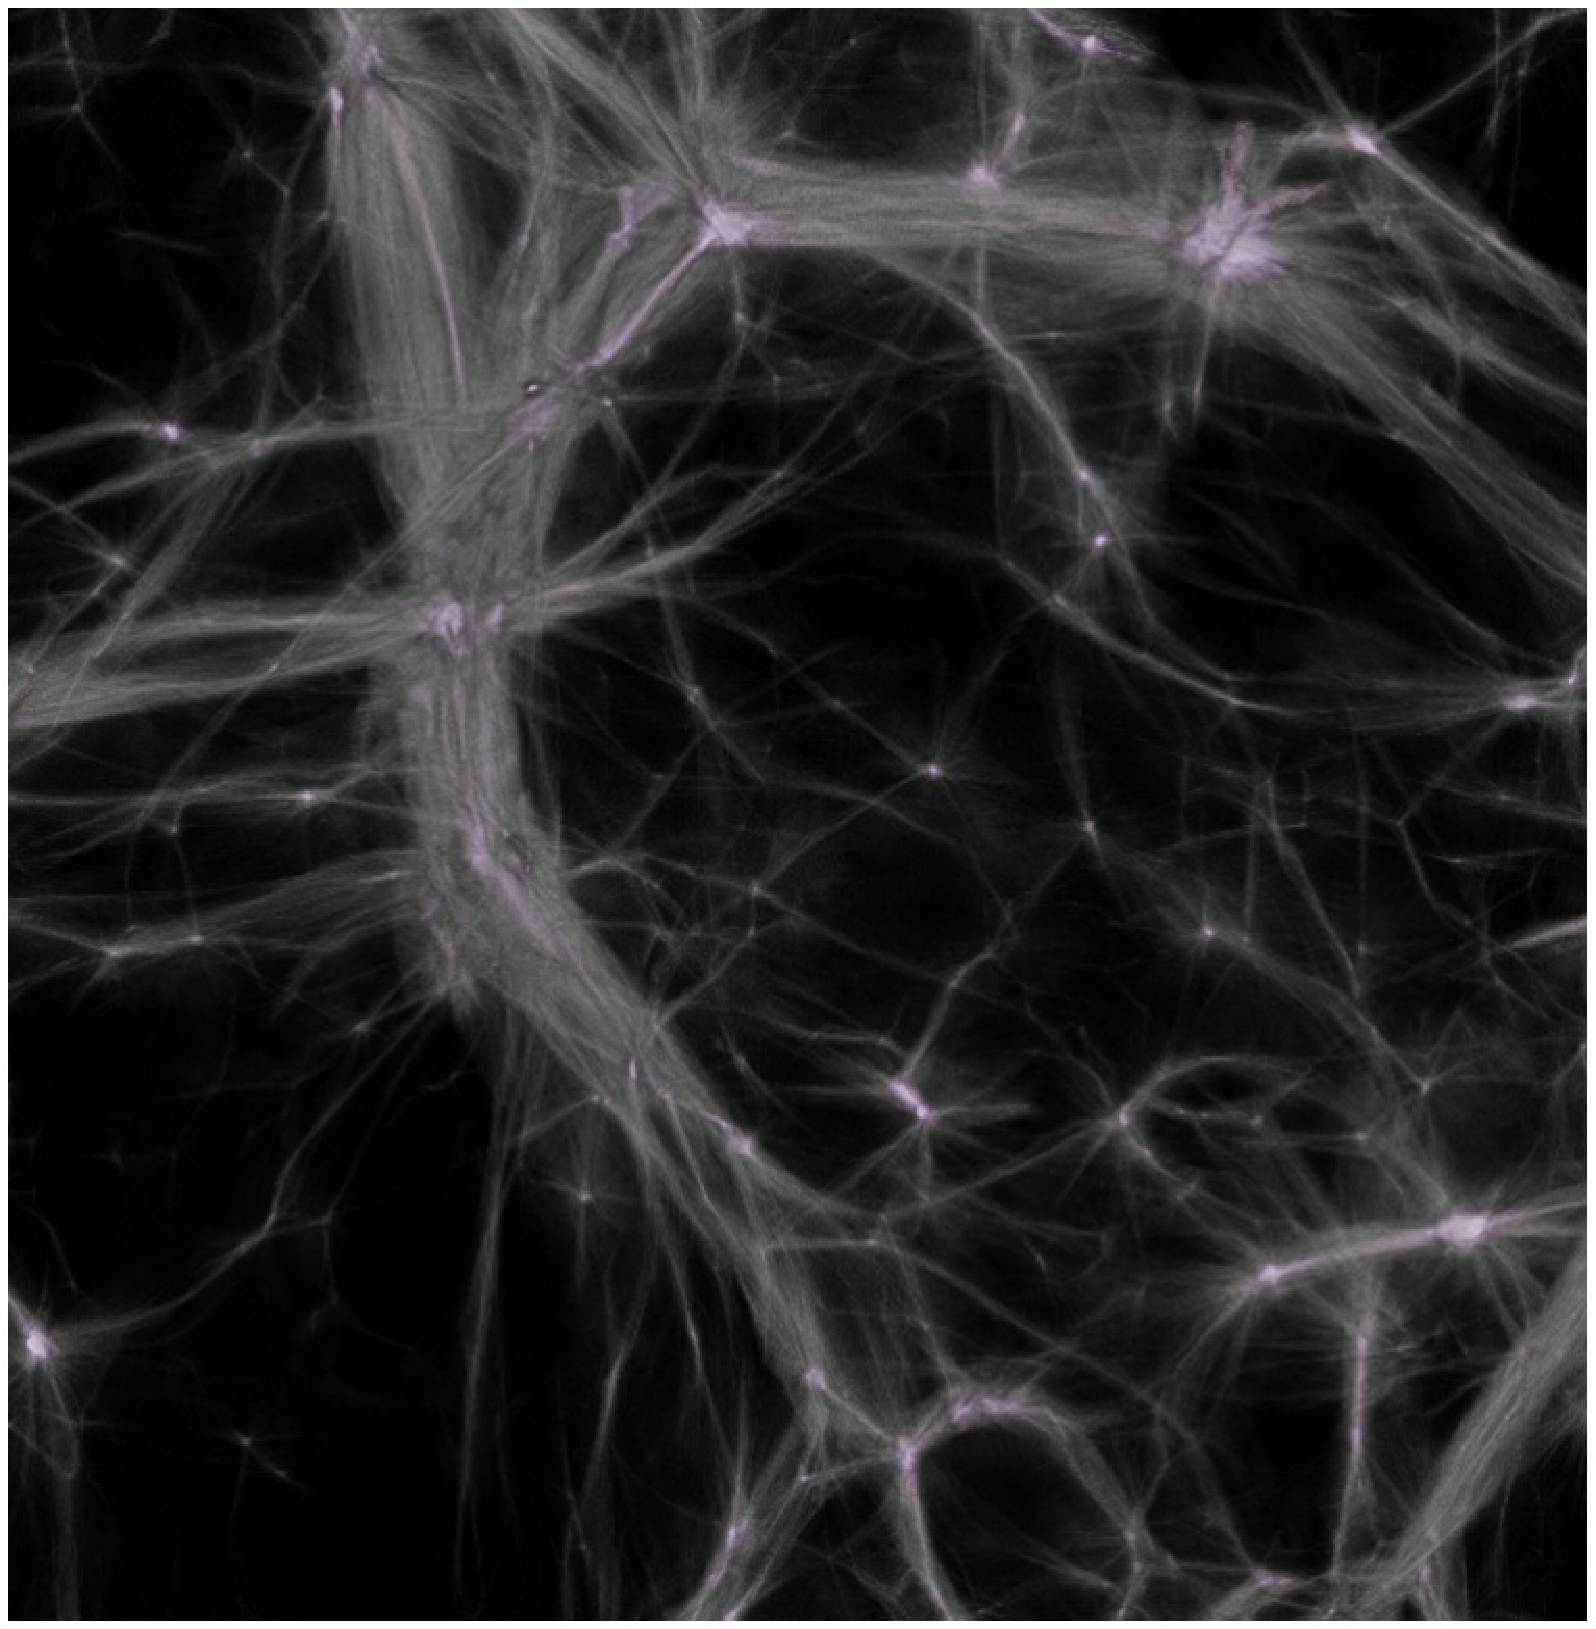
\includegraphics[width=16cm]{Chapter4/Source_v2/fig1.pdf} 
\caption{3D rendering of the multistream field: the cosmic web structure of a $ 50 h^{-1} \text{Mpc} \times 50 h^{-1} \text{Mpc} \times 50 h^{-1} \text{Mpc}$ slice in a simulation box of side length $100 h^{-1}$ Mpc and $128^3$ particles. The multistream field is calculated at 8 times the native resolution. void(black) is a percolating structure with $n_{str} = 1$. Regions $n_{str} \geq 17$ show a filamentary structure (gray) and the bright spots at the intersections of the filaments are regions with $n_{str} \geq 100$. }
\label{fig:full_3d}
\end{figure}

In three-dimensional simulations, the Lagrangian sub-manifold twists in complicated ways in a six-dimensional phase space. This is due to complexities involving caustic formations in higher dimensions, which is true even in the ZA, see \citealt{Arnold1982} and \citealt{Hidding2014} for detailed analyses of caustic formation. The resulting intricate geometrical structures can be characterized by the $n_{str}$ field. Nearly  $90\%$ of the volume in N-body simulations are single-streamed voids at $z=0$ (\citealt{Shandarin2012}, also see \citealt{Falck2015} for a percolation analysis of single-streaming voids). From the visualizations in \cite{Ramachandra2015} and percolation analysis of \cite{Ramachandra2017}, we also know that the $n_{str} = 3$ regions mostly form connected wall-like structures (also see \autoref{fig:full_3d}), unlike the isolated patches as seen in one-dimensional simulations of \autoref{fig:1d}. The structures become predominantly filamentary at higher thresholds of $ n_{str} \gtrsim 17$. Subsequently, the regions around the multistream maxima have isolated closed surfaces (for example, in \autoref{fig:full}), which may be identified as halo locations. 



\begin{figure} 
\centering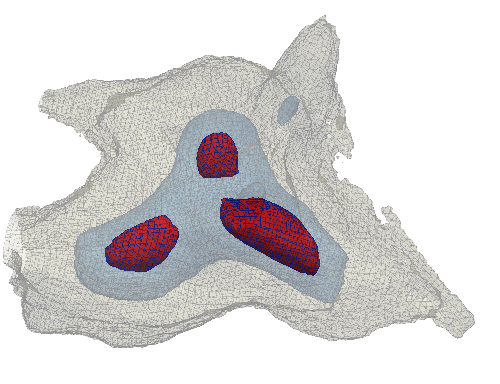
\includegraphics[width=11cm]{Chapter5/Source_v2/fig2.pdf} 
\caption{Multistream field contours: The multistream field is calculated at 8 times the native resolution. Each inner convex blobs (red) surround local multistream maxima inside. Surrounding outer shell(blue) is not convex throughout the surface, and the outermost gray multistream surface displays a filamental geometry.}
\label{fig:full}
\end{figure}


Caustic formations and mass accretion are also seen to occur more along the higher streams, which makes the haloes non-spherical, with the alignment generally determined by a complicated interplay  of the intensities of the streams from neighboring filamentary structures. Number of streams corresponding to the dark matter halo also has a local environment dependence. The three small haloes in \autoref{fig:full}, where the number of streams are higher than the neighbouring filaments, are aligned along three intersecting filaments. Halo environment studied in \cite{Ramachandra2015} show similar hierarchical variation in $n_{str}$ values. The halo environments are thus very complicated, and empirical thresholds (on multistream or density fields) may not account for all the haloes uniformly. Hence we use a local geometrical method to identify potential haloes in multistream fields.


The first non-linear structures in the web have $n_{str} = 3$. By visual inspection, these regions generally form a fabric-like open structures that resemble walls. The surface contours of higher $n_{str}$ are embedded within the walls. \autoref{fig:full_3d} shows a filamentary structure of the web at $n_{str} \gtrsim 17$. The figure also shows regions around local maxima of the multistream field, which are generally located at the intersections of filaments.    








% % \section{Dynamics: Lagrangian sub-manifold}
% Multi-stream flows, Caustics, Flip-flips